\documentclass[10pt,twocolumn]{article}
\usepackage[margin=0.8in]{geometry}
\usepackage{mathptmx}
\usepackage{amsmath}
\usepackage{booktabs}
\usepackage{graphicx}
\usepackage[numbers,sort&compress]{natbib}
\usepackage[hidelinks]{hyperref}
\usepackage{fontspec}
\newfontfamily\kofont{WenQuanYi Zen Hei}
\setlength{\columnsep}{0.25in}

\title{\textbf{ART FARM: Field-Scale Water-Risk Screening for Corn Belt Crop Rotation Using NASA Earth Observations}}
\author{Team Amolla ({\kofont 아몰라})\\NASA Space Apps Challenge 2026 Seoul}
\date{}

\begin{document}
\maketitle
\renewcommand{\thefootnote}{}
\footnotetext{Drafted with SI (Claude Code and open-source writing tools) from the team's own results; all numbers come from the ART FARM engine and team MATLAB validation; all references verified via OpenAlex.}
\renewcommand{\thefootnote}{\arabic{footnote}}

\begin{abstract}
Corn Belt farmers choose crop rotations under growing weather and water risk, but most decision aids give either regional averages or a single deterministic forecast. ART FARM is a two-tier screening tool. A \emph{Quick Screen} tier works anywhere in the Corn Belt from ten years of NASA POWER weather, USGS elevation and FAO-56 crop-water formulas and labels every output a ``screening estimate''. A \emph{Deep Analysis} tier runs a daily FAO-56 soil-water balance over 500 resampled weather seasons for 20 pilot fields in four counties (Story IA, McLean IL, Lancaster NE, Union OH) and compares four strategies: corn--soybean (A), plus a cereal-rye cover (B), plus a small grain (C) and plus alfalfa (D). Results are reported as P10--P90 ranges with a worst-10\% tail (CVaR\textsubscript{10}), a replay of the 2012 drought, and seasonal and climate ranges from NASA GEOS-S2S and NEX-GDDP-CMIP6. For one Story County field the strategy-A growing-season water deficit is 115/188/265\,mm (P10/P50/P90; CVaR\textsubscript{10} 301\,mm), and its 2012 replay deficit is 463\,mm (A), 451\,mm (B), 366\,mm (C) and 513\,mm (D). Team MATLAB checks show that the four counties' 2012 deficits move in the same direction as USDA NASS yield losses (corn $r=-0.49$, soybean $r=-0.85$, $n=4$ counties, $p\approx0.15$ for soybean, not significant), that a $\pm$10\% change in crop coefficients shifts deficits by $-19.2$\% to $+21.1$\% without changing any strategy ranking (0 of 80 cases), and that the Prithvi geospatial foundation model's majority class matches the USDA Cropland Data Layer on 19 of 20 fields. Decision support only --- does not replace farmer judgment.
\end{abstract}

\section{Introduction}
U.S. maize production has become more sensitive to drought as yields have risen \citep{lobell2014}, and temperature extremes cause sharply nonlinear yield damage \citep{schlenker2009}. Climate variation explains about a third of global yield variability \citep{ray2015}, and new-generation climate and crop-model ensembles show that impacts emerge earlier than previously projected \citep{jagermeyr2021,rosenzweig2014,hatfield2011}. At the same time, rotation choice shapes both yield and resilience: continuous corn and continuous soybean carry measurable yield penalties across hundreds of thousands of fields \citep{seifert2017}, and diversified rotations increase maize yields and reduce drought losses \citep{bowles2020}.

Farmers therefore need a field-level answer to a narrow question: \emph{under the range of weather this field could plausibly see, how do candidate rotations differ in water stress?} ART FARM addresses this with NASA Earth observations and a transparent FAO-56 water balance. Its design rules are: (i) ranges, never single forecasts; (ii) every number traceable to an engine response or a validation artifact; (iii) every card lists drawbacks, information gaps and a reminder to confirm with a field soil test. The tool does not tell a farmer what to plant.

\section{Related Work}
\textbf{Crop water balance.} The FAO-56 approach estimates crop evapotranspiration from reference evapotranspiration and stage-dependent crop coefficients; standard single and basal coefficients were recently updated \citep{pereira2021}. AquaCrop extends this to water-driven yield simulation \citep{steduto2009,raes2009}, with maize parameterisation documented by \citet{hsiao2009}. ART FARM uses the FAO-56 bucket for stress screening only; it does not simulate yield.

\textbf{Remote-sensing evapotranspiration.} Energy-balance methods such as METRIC \citep{allen2007}, ALEXI \citep{anderson2007} and SSEBop \citep{senay2013} map actual ET from satellites; OpenET combines an ensemble of such models for field-scale water management \citep{melton2022}. Global requirements for ET observations are reviewed by \citet{fisher2017}.

\textbf{Rotation and conservation effects.} Beyond yield \citep{seifert2017,bowles2020}, cover crops can sequester soil carbon \citep{poeplau2015,lal2004} and reduce nitrate leaching relative to bare fallow \citep{tonitto2006}. Soybean biological N fixation supplies a large share of crop N \citep{salvagiotti2008}, whereas synthetic N fertilizer is a major source of crop-production greenhouse-gas emissions \citep{snyder2009}.

\textbf{Risk metrics.} Conditional value-at-risk (CVaR) summarises the mean of the worst tail of a distribution and is widely used in risk optimisation \citep{rockafellar2000}.

\section{Data}
Table~\ref{tab:data} lists the datasets. Daily weather comes from NASA POWER \citep{sparks2018}, whose meteorology derives from the MERRA-2 reanalysis \citep{gelaro2017}. Soil moisture comes from SMAP \citep{entekhabi2010,ds_smap}; precipitation from GPM IMERG \citep{hou2014,ds_imerg}; surface reflectance and NDVI from Harmonized Landsat--Sentinel-2 \citep{claverie2018,ds_hlsl30,ds_hlss30}; land-surface forcing from NLDAS-2 \citep{xia2012,ds_nldas}; and field ET context from OpenET \citep{melton2022}. Next-season ranges use GEOS-S2S \citep{molod2020} and multi-decade ranges NEX-GDDP-CMIP6 \citep{thrasher2022,ds_nexgddp}. Crop labels are cross-checked with the Prithvi geospatial foundation model \citep{jakubik2023,ds_prithvi}. USDA layers provide crop history (Cropland Data Layer, CDL \citep{boryan2011}), field polygons (Crop Sequence Boundaries, CSB), county yields (NASS Quick Stats) and soils (NRCS SSURGO).

\begin{table}[t]
\centering\small
\caption{Data sources used by the engine and validation.}
\label{tab:data}
\begin{tabular}{@{}ll@{}}
\toprule
Dataset & Role \\
\midrule
NASA POWER (daily) & weather, ET\textsubscript{0} \\
SMAP L3 enhanced & root-zone moisture context \\
GPM IMERG Final V07 & precipitation check \\
HLS L30/S30 v2.0 & NDVI, bare-soil days \\
NLDAS-2 forcing & 2012 cross-check \\
OpenET & ET context \\
GEOS-S2S & next-season ensemble \\
NEX-GDDP-CMIP6 & climate-epoch ranges \\
Prithvi-100M crop class. & crop-label check \\
USDA CDL / CSB & crop history, fields \\
USDA NASS Quick Stats & county yields \\
USDA NRCS SSURGO & soil water capacity \\
\bottomrule
\end{tabular}
\end{table}

\section{Methods}
\textbf{Quick Screen.} The user clicks four field corners; the browser pulls ten years of NASA POWER weather and USGS 3DEP elevation and applies FAO-56 formulas. The user picks two or three of corn, soybean and wheat; rotations are shown without ranking and labelled ``screening estimate''. The code is a JavaScript port of the team's MATLAB prototype (V8).

\textbf{Deep Analysis engine.} For each pilot field a daily soil-water bucket with FAO-56 water stress and SCS curve-number runoff is run over 500 resampled weather sequences (1995--2025 POWER weather) with a fixed seed. All strategies share the same weather draws, so differences come from the rotation rather than sampling luck. Each metric (growing-season water deficit, stress days, drainage, winter bare days, etc.) is returned as P10/P50/P90 and CVaR\textsubscript{10}, the mean of the worst 10\% of samples \citep{rockafellar2000}. Seasonal (GEOS-S2S, 10 members) and climate (NEX-GDDP-CMIP6) scenarios are reported as separate ranges, never as a single forecast.

\textbf{2012 backtest.} A deterministic water balance is driven by the actual POWER weather of 2012 with three spin-up years (2009--2011). Strategy A uses the observed CDL crops; B adds cereal rye; C and D are means over rotation phases.

\textbf{Independent team checks (MATLAB).} Four team members ran MATLAB (R2026b) analyses on engine outputs: county yield comparison with NASS, HLS NDVI bare-soil days, crop-coefficient sensitivity, and a batch run of the V8 prototype (20/20 fields, 80 rows, 0 failures).

\section{Results}
\textbf{Pilot fields.} The 20 pilot fields are in Story IA (12), McLean IL (3), Lancaster NE (3) and Union OH (2).

\textbf{Example field.} For Story County field 191825003869023 (corn--soybean), the strategy-A growing-season water deficit over 500 resampled seasons is P10 115\,mm, P50 188\,mm, P90 265\,mm, with CVaR\textsubscript{10} 301\,mm. With the next-season GEOS-S2S ensemble (10 members) the P10--P90 range shifts to 136--309\,mm.

\textbf{2012 backtest.} For the same field the 2012 season deficit is 462.8\,mm (A), 450.9\,mm (B), 365.6\,mm (C) and 512.9\,mm (D); strategy A shows 88 stress days. Figure~\ref{fig:backtest} shows the replay for three McLean IL fields, whose bars match the live model API.

\begin{figure}[t]
\centering
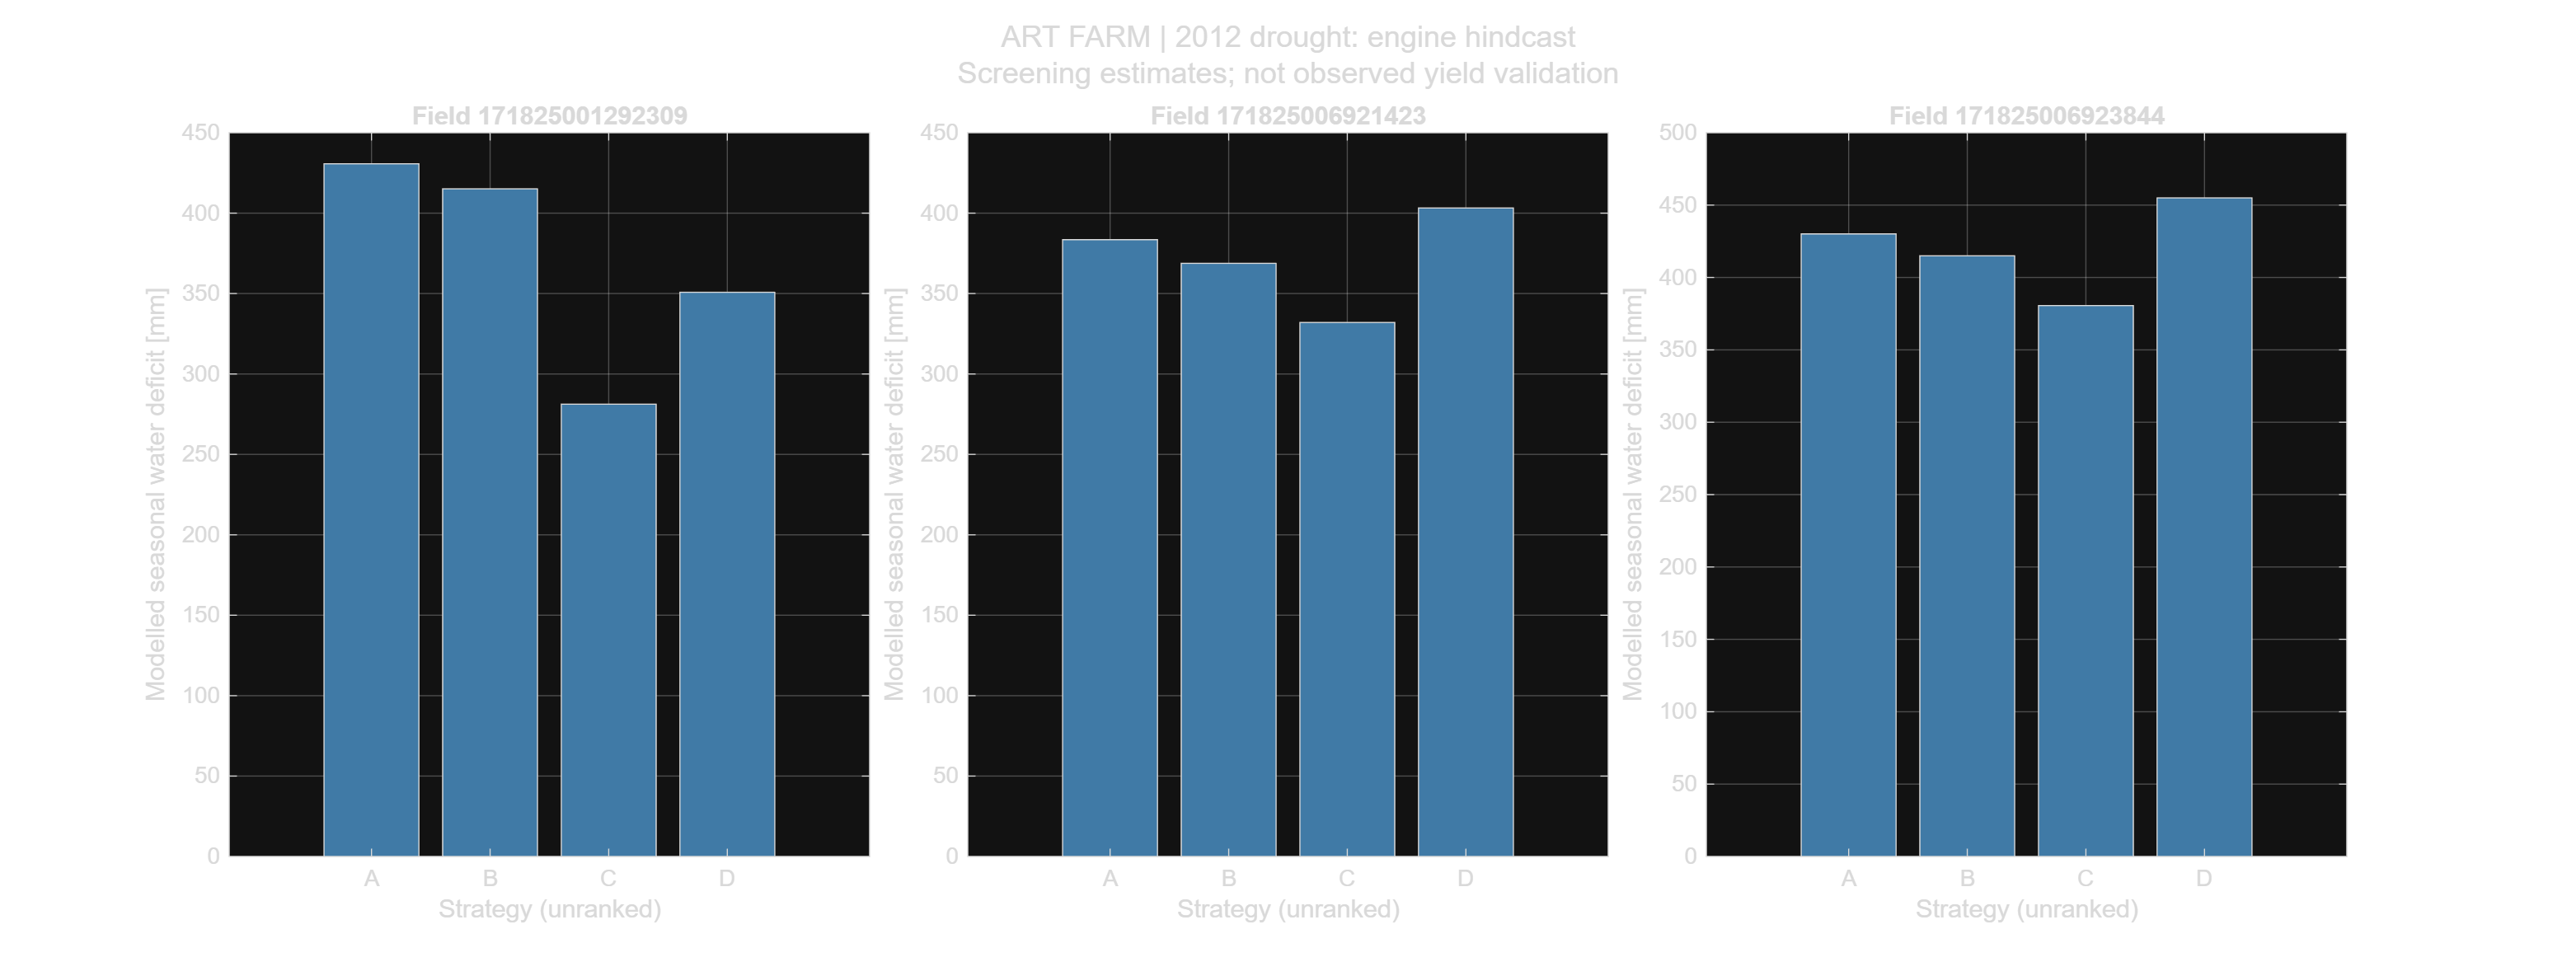
\includegraphics[width=\columnwidth]{figs/fig_backtest2012.png}
\caption{2012 drought replay: season water deficit by strategy for three McLean IL pilot fields (team MATLAB plot of engine output).}
\label{fig:backtest}
\end{figure}

\textbf{NASS county comparison.} Table~\ref{tab:nass} compares 2012 county yields with each county's 2001--2024 baseline (excluding 2012 and 2025) and the mean engine 2012 deficit over that county's pilot fields. All four counties had below-baseline yields. Correlation of deficit with yield change is $r=-0.49$ for corn and $r=-0.85$ for soybean with $n=4$ counties per crop; the soybean value gives $p\approx0.15$, so neither is statistically significant (Spearman $\rho = 0$ and $-0.4$). The MATLAB cross-check of engine deficit against POWER May--September precipitation anomaly gives $r=-0.87$ ($n=4$); this uses the same POWER data and is not an independent validation. These are directional sanity checks only; yield is not the engine objective.

\begin{table}[t]
\centering\small
\caption{2012 NASS yield change vs.\ engine deficit (strategy A).}
\label{tab:nass}
\begin{tabular}{@{}lrrrr@{}}
\toprule
County & Corn & Soy & Deficit & Fields\\
 & chg. & chg. & (mm) & \\
\midrule
Story IA & $-13.0$\% & $-5.9$\% & 469.9 & 12\\
McLean IL & $-44.0$\% & $-11.9$\% & 414.8 & 3\\
Lancaster NE & $-42.6$\% & $-43.7$\% & 643.3 & 3\\
Union OH & $-18.1$\% & $-8.8$\% & 306.5 & 2\\
\bottomrule
\end{tabular}
\end{table}

\begin{figure}[t]
\centering
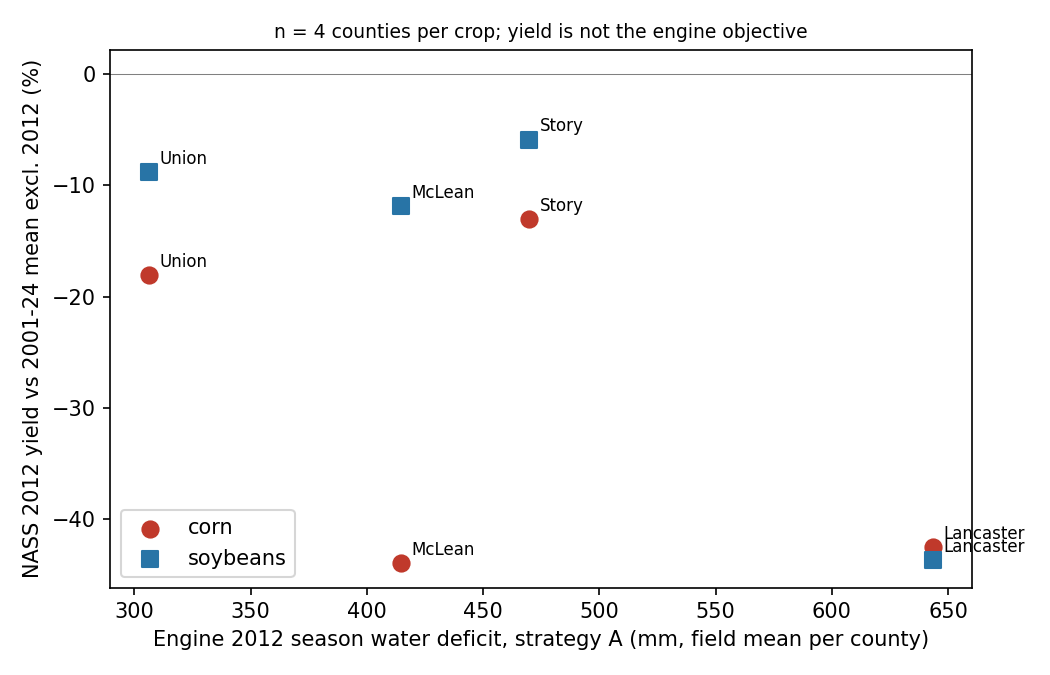
\includegraphics[width=\columnwidth]{figs/nass_2012_vs_engine.png}
\caption{2012 county yield change (USDA NASS) vs.\ engine water deficit; $n=4$ counties, directional only.}
\label{fig:nass}
\end{figure}

\textbf{NDVI and bare soil.} From HLS NDVI for 2023--2025 (60 field-years, 20 fields), median winter low-NDVI (bare) days were 29.5 in 2024 (range 10--55) and 44.5 in 2025 (range 23--55); 2023 has one missing field. Mean observation coverage per year was 0.57--0.60. NDVI anomaly was not correlated with season water deficit ($r=-0.09$, $p=0.498$, $n=60$), nor was season length ($r=0.00$, $p=0.988$, $n=55$). HLS does not overlap 2012, so no 2012 NDVI comparison was made.

\textbf{Kc sensitivity.} Changing all crop coefficients by $-10$\% and $+10$\% for 80 field--rotation cases (20 fields $\times$ 4 V8 rotations) changed the deficit by $-19.21$\% to $-17.24$\% and $+18.27$\% to $+21.06$\% respectively, i.e.\ roughly twice the coefficient change, and changed the rotation ranking in 0 of 80 cases. Absolute deficits are therefore coefficient-sensitive, while relative comparisons are robust to this perturbation.

\textbf{Prithvi agreement.} For 2024, Prithvi's most common class matched the CDL crop on 19 of 20 pilot fields; per-field pixel agreement ranged from 0.193 to 0.997 (median 0.934, mean 0.883). Most pilot fields are uniform corn or soybean, so this is not a general accuracy figure (model card: 60.64\% aAcc).

\section{Interpretation}
The following subsections are qualitative; they introduce no new numbers.

\subsection{Agricultural economics}
Weather drives a large share of yield variability \citep{ray2015,schlenker2009}, so a farmer's income risk is concentrated in bad years. Reporting P10--P90 and CVaR\textsubscript{10} rather than a mean lets a farmer compare rotations by their downside, the quantity that matters for liquidity, crop insurance and credit. The 2012 replay gives a concrete stress test that farmers and insurers already recognise.

\subsection{Business}
The value of a screening tool lies in narrowing options cheaply before costly agronomic advice. The scaling path follows the two tiers: Quick Screen runs anywhere from public NASA data with no account, while Deep Analysis extends county by county as CSB, SSURGO and engine runs are added. Partners such as extension services, crop advisers and conservation programmes are natural channels.

\subsection{Energy}
Higher water deficits imply more irrigation pumping energy where irrigation is available. Synthetic N fertilizer carries substantial production energy and emissions \citep{snyder2009}, whereas soybeans obtain much of their N by biological fixation \citep{salvagiotti2008}; rotations including legumes can therefore reduce the fertilizer energy embedded in a farm's inputs. ART FARM does not yet quantify either term.

\subsection{Environment}
Cover crops and diversified rotations can raise soil organic carbon \citep{poeplau2015,lal2004} and reduce nitrate loss compared with bare fallow \citep{tonitto2006}. Winter bare-soil days, which the engine and the HLS analysis both track, are a direct indicator of the window in which such losses occur. Strategy B's lower 2012 deficit for the example field is consistent with, but does not prove, a water benefit from residue cover.

\subsection{Policy}
U.S. conservation programmes---USDA climate-smart commodity partnerships, NRCS EQIP and CSP, and conservation funding expanded under the Inflation Reduction Act---pay for practices such as cover crops and conservation rotations. NASA Earth Science Applied Sciences and its agriculture consortium (NASA Acres) aim to put satellite data into such decisions. A transparent, field-scale screening layer could help farmers and programme staff discuss practice choices with shared evidence; it is not a basis for eligibility or payment.

\subsection{Climate adaptation and resilience}
Climate impacts on crops are expected to intensify \citep{jagermeyr2021,rosenzweig2014,hatfield2011}. Presenting seasonal (GEOS-S2S) and climate (NEX-GDDP-CMIP6) ranges side by side with a historical stress year helps farmers see adaptation as risk management rather than prediction.

\section{Limitations}
(i) The engine does not model rotation order effects on yield (e.g.\ the rotation benefits in \citep{seifert2017,bowles2020}); C and D are phase means. (ii) Validation samples are small: $n=4$ counties for NASS, 20 fields overall; no correlation reported here is statistically significant. (iii) Field resolution is limited: POWER, SMAP, GEOS-S2S and CMIP6 grids are much coarser than a field, and HLS observation coverage averaged under 61\%. (iv) The 2012 county cross-check reuses POWER and is not independent. (v) All outputs are screening estimates; V8 economic and index coefficients are unvalidated, and Quick Screen uses a simplified ET\textsubscript{0} proxy rather than full Penman--Monteith.

\section{Future Work}
Independent validation against OpenET actual ET \citep{melton2022} and SMAP soil moisture at more fields; AquaCrop-style yield response \citep{steduto2009}; rotation order effects; more counties to raise $n$; and quantified energy and nitrate indicators.

\section{Conclusion}
ART FARM shows that public NASA Earth observations and an FAO-56 water balance can give Corn Belt farmers field-scale, range-based water-risk screening for rotation choices, with every number traceable to an engine response or a team validation artifact. Early checks are directionally consistent with 2012 county yield losses and robust in ranking to $\pm$10\% coefficient changes, but they are small-sample and not statistically conclusive. Decision support only --- does not replace farmer judgment.

\small
\bibliographystyle{plainnat}
\bibliography{references}
\end{document}
